
%
%	Simulation
%

\section{Simulation}\label{Section_Simula}
\Headerfooter{Simulation}

\subsection{Atmospheric neutrino flux}
\vs\hs Atmospheric neutrino flux!

\begin{figure}[tbp]
	\centering
	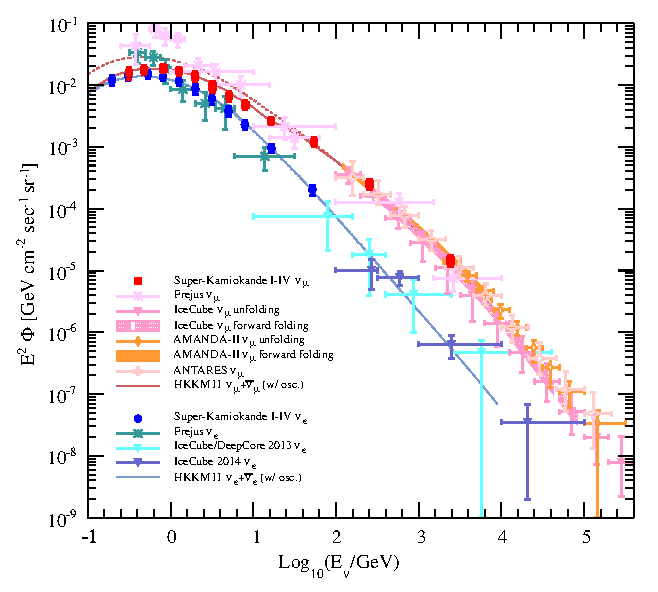
\includegraphics[width=12cm]{Figures/Simulation/AtmNeuFlux}
	\caption[HKKM11 atmospheric neutrino flux model predictions for the Kamioka site and the measured energy spectra of the atmospheric $\nu_{\text{e}}$ and $\nu_{\mu}$ fluxes by some experiments]{\label{Simula_AtmNeuFlux} HKKM11 atmospheric neutrino flux model predictions for the Kamioka site and the measured energy spectra of the atmospheric $\nu_{\text{e}}$ and $\nu_{\mu}$ fluxes by some experiments~\cite{2011Honda,2016Richard}.}
\end{figure}

\begin{figure}[tbp]
	\centering
	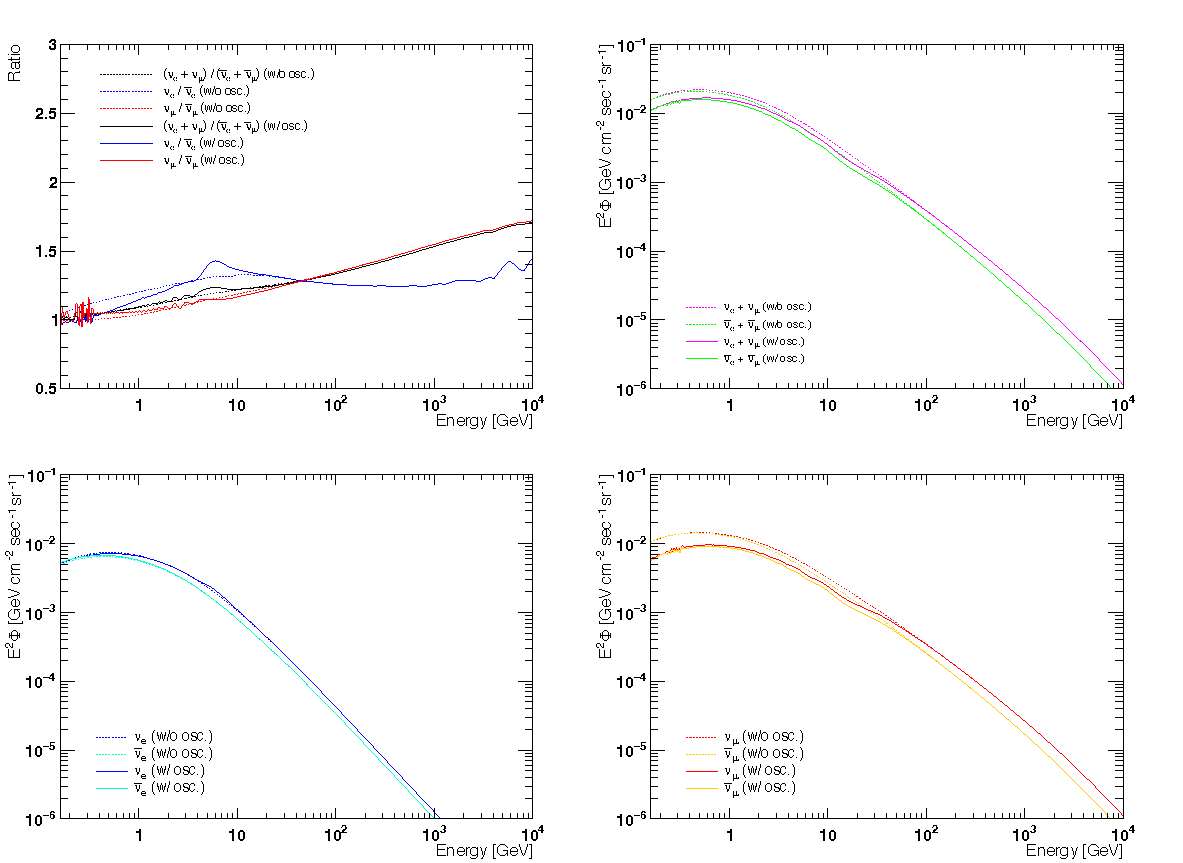
\includegraphics[width=14cm]{Figures/Simulation/Ratio}
	\caption[Atmospheric neutrino-antineutrino flux ratio predicted by the HKKM11 model for the Kamioka site]{\label{Simula_Ratio} Atmospheric neutrino-antineutrino flux ratio predicted by the HKKM11 model for the Kamioka site (top left)~\cite{2011Honda}. Atmospheric neutrino fluxes of $\nu_{\text{e}}\,+\,\nu_{\mu}$ ($\bar{\nu}_{\text{e}}\,+\,\bar{\nu}_{\mu}$) (top right), $\nu_{\text{e}}$ ($\bar{\nu}_{\text{e}}$) (bottom left), and $\nu_{\mu}$ ($\bar{\nu}_{\mu}$) (bottom right) are also shown.}
\end{figure}

\subsection{Neutrino interaction}
\vs\hs Neutrino interaction!

\begin{figure}[tbp]
	\centering
	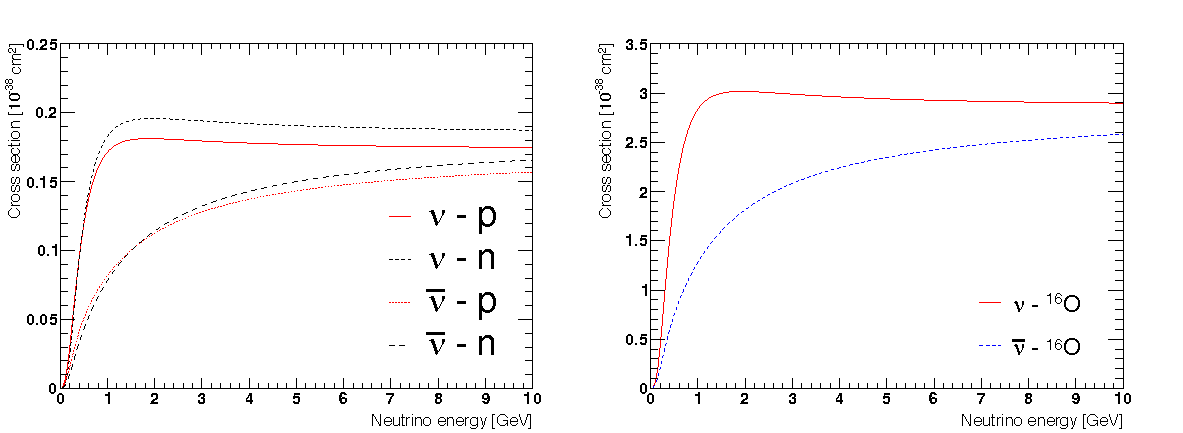
\includegraphics[width=14cm]{Figures/Simulation/NCQECroSec}
	\caption[NCQE cross section on nucleon and on oxygen nucleus]{\label{Simula_NCQECroSec} NCQE cross section on nucleon (left) and on oxygen nucleus (right)~\cite{2012Ankowski}.}
\end{figure}

\begin{figure}[tbp]
	\centering
	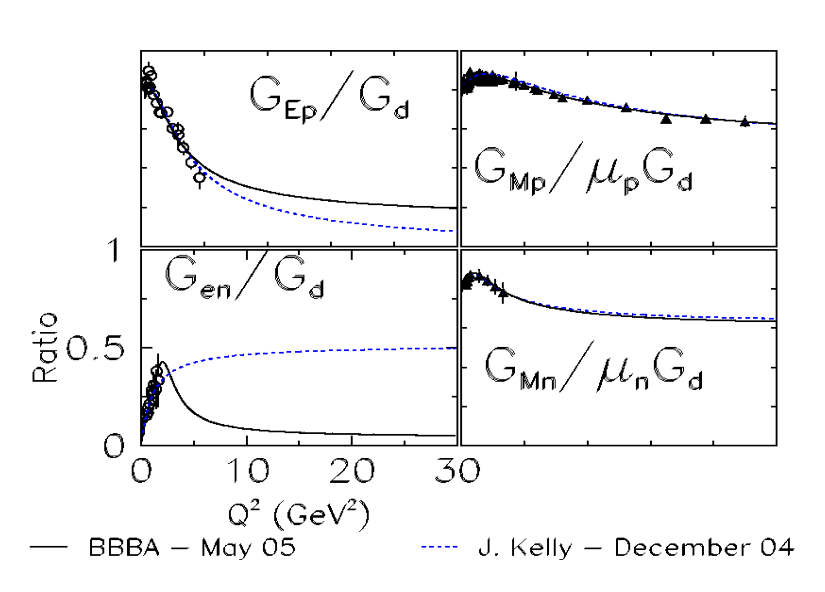
\includegraphics[width=10cm]{Figures/Simulation/BBBA05}
	\caption[Ratio of the BBBA05 form factors to $G_{d}$]{\label{Simula_BBBA05} Ratio of the BBBA05 form factors to $G_{d}$ (the dipole form factor) (shown in the solid brack line)~\cite{2006Bradford}. The dashed blue line shows the ratio of the Kelly form factors to $G_{d}$.}
\end{figure}

\subsection{Simulation for the IBD-like event}
\vs\hs Simulation for the IBD-like event!

\subsection{Detector simulation}
\vs\hs Detector simulation!

\begin{figure}[tbp]
	\centering
	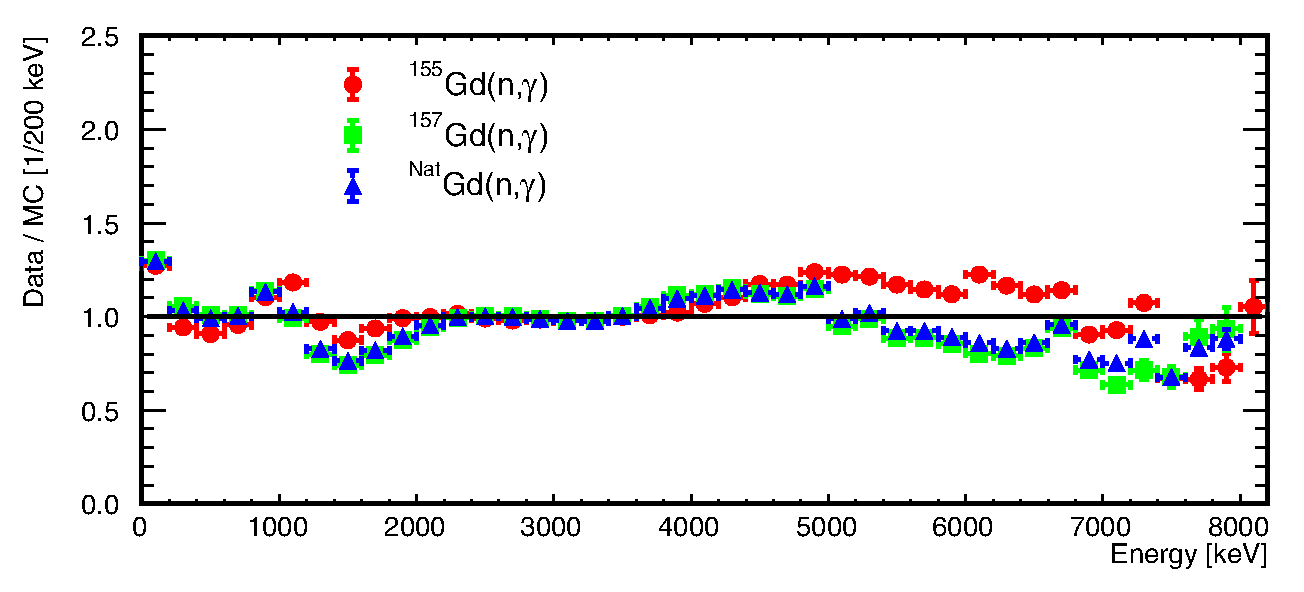
\includegraphics[width=10cm]{Figures/Simulation/RatioGdGam}
	\caption[Ratio of data from the ANNRI experiment by MC with the ANNRI-Gd model for the single gamma-ray events]{\label{Simula_RatioGdGam} Ratio of data from the ANNRI experiment to MC with the ANNRI-Gd model for the single gamma-ray events~\cite{2020Tanaka}.}
\end{figure}

\newpage
